% =============================================================================
%  Bilibili User Personality Analysis
%  A Research Prototype for Argumentative-Behavior Risk Assessment
%  on Chinese Social Media Platforms
% =============================================================================

\documentclass[11pt,a4paper]{article}

% --- Page layout ---
\usepackage[margin=1in]{geometry}
\usepackage{setspace}
\onehalfspacing

% --- Fonts & encoding ---
\usepackage[T1]{fontenc}
\usepackage[utf8]{inputenc}
\usepackage{newtxtext,newtxmath}

% --- Graphics ---
\usepackage{graphicx}
\usepackage{tikz}
\usetikzlibrary{arrows.meta,shapes,positioning,fit}

% --- Math & symbols ---
\usepackage{amsmath,amssymb,amsthm}
\usepackage{bm}

% --- Tables ---
\usepackage{booktabs}
\usepackage{array}
\usepackage{longtable}

% --- Captions & floats ---
\usepackage{caption}
\usepackage{subcaption}

% --- Hyperlinks ---
\usepackage[colorlinks=true,linkcolor=blue,citecolor=blue,urlcolor=blue]{hyperref}

% --- Bibliography ---
\usepackage[backend=biber,style=ieee,sorting=nyt]{biblatex}
\addbibresource{references.bib}

% --- Code listings ---
\usepackage{listings}
\lstset{
  basicstyle=\ttfamily\small,
  breaklines=true,
  frame=single,
  numbers=left,
  numberstyle=\tiny,
  captionpos=b
}

% --- Theorem environments ---
\newtheorem{definition}{Definition}[section]
\newtheorem{remark}{Remark}[section]

% --- Metadata ---
\title{
  \textbf{Bilibili User Personality Analysis}\\[4pt]
  \large A Research Prototype for Argumentative-Behavior Risk Assessment\\
  on Chinese Social Media Platforms
}

\author{
  JunWeiLi233\\
  \texttt{https://github.com/JunWeiLi233/Bilibili\_User\_Personality}
}

\date{\today}

\begin{document}
\maketitle

% =============================================================================
\begin{abstract}
This paper presents a research prototype for evaluating argumentative-behavior risk in
Chinese-language online discourse. The system analyzes public comments, replies, and
danmaku (bullet-screen comments) from the Bilibili video platform to produce a
multi-dimensional behavioral profile for individual users. The analysis rests on three
interlocking components: (1) a six-axis behavioral scoring framework grounded in
argumentation theory and the psychology of online discourse, (2) an auditable
Chinese internet-slang dictionary with 4,956 entries organized into six semantic
families, each backed by Bilibili-sourced evidence, and (3) three iterative coverage
loops---corpus mining, local expansion, and auto-coverage harvesting---that
progressively close the evidence gap through a combination of offline text matching and
live API-driven comment collection validated by large language models. The system
produces a radar chart, a composite trolling index, and sentence-level diagnostic output
for each analyzed user. We describe the architecture, the dictionary construction
pipeline, the coverage-driven quality mechanism, and current limitations. The prototype
is released as open-source software under the MIT License.
\end{abstract}

% =============================================================================
\section{Introduction}

Online discourse on Chinese social media platforms exhibits a distinctive set of
argumentative behaviors that differ from those observed in English-language contexts.
On Bilibili---a platform with over 300 million monthly active users---public discussion
often features \textit{passive-aggressive rhetoric}, \textit{absolute quantification},
\textit{burden-of-proof shifting}, and \textit{categorical refusal to correct errors}
when confronted with counter-evidence. These behaviors, colloquially referred to as
``杠精'' (\textit{gang jing}, or ``argumentative troll''), are not captured by
existing toxicity-detection models trained on English corpora, nor by lexicon-based
Chinese sentiment analyzers that lack context-aware semantic judgment.

This project addresses a bounded research question: \textbf{given a Bilibili user's
publicly available comment history, can we produce a reliable, evidence-backed assessment
of their argumentative-behavior risk across multiple interpretable dimensions?}
The output is explicitly framed as a behavior-risk analysis over a limited public sample,
not as a clinical diagnosis or definitive personality judgment.

The contribution of this work is threefold:
\begin{enumerate}
  \item A \textbf{six-dimensional behavioral scoring framework} tailored to
    Chinese-language argumentative discourse, with each dimension scored 0--100 and
    backed by at least one quoted comment from the analyzed user.
  \item An \textbf{auditable dictionary} of 4,956 Chinese internet-slang terms organized
    into six semantic families, each requiring a minimum of three pieces of
    Bilibili-sourced evidence before contributing full weight to the final score.
  \item Three \textbf{iterative coverage-loop mechanisms} that progressively populate
    the dictionary with real-world evidence through a combination of offline text
    matching and live API-driven harvesting validated by DeepSeek V4.
\end{enumerate}

The remainder of this paper is organized as follows. Section~2 surveys related work.
Section~3 defines the six behavioral dimensions and the scoring methodology.
Section~4 describes the dictionary system and coverage mechanism.
Section~5 details the coverage loops.
Section~6 presents the system architecture.
Section~7 discusses current status and limitations.
Section~8 outlines future work, and Section~9 concludes.


% =============================================================================
\section{Related Work}

\subsection{Toxicity Detection in Social Media}

Conventional toxicity detection systems~\cite{davidson2017automated,founta2018unified}
classify text into broad categories (toxic, severe toxic, obscene, threat, insult,
identity hate) using supervised classifiers trained on crowd-annotated datasets.
While effective for English-language social media, these systems are poorly calibrated
for Chinese internet discourse, where toxicity frequently manifests through
\textit{semantic indirection}---sarcasm, allusion, inverted meaning, and meme-dense
language---rather than through explicit profanity.

\subsection{Chinese NLP for Social Media}

Chinese-specific NLP work has made significant
progress in word segmentation, named-entity recognition, and sentiment analysis.
However, most existing Chinese sentiment lexicons (e.g., NTUSD~\cite{ku2007mining},
HowNet~\cite{dong2006hownet}) are designed for general-domain text and fail to capture
the fluid, rapidly evolving internet slang that characterizes Bilibili discourse.
Bilibili-specific NLP work is scarce, partly because the platform's public API imposes
strict rate limits and the danmaku comment format---short, context-dependent, often
ironic---poses unique challenges for conventional NLP pipelines.

\subsection{Argumentation Mining}

Argumentation mining~\cite{stede2018argumentation,peldszus2013argument} aims to
automatically identify argumentative structures in text: claims, premises, conclusions,
and attack/support relations. Our work draws on this tradition but applies it at a
coarser granularity: rather than reconstructing full argumentation trees, we score
six behavioral dimensions that proxy for argumentative quality. This pragmatic approach
reflects the constraints of real-world deployment---short comments, noisy text, and
platform-specific linguistic conventions.

\subsection{LLM-Assisted Content Analysis}

Recent work demonstrates that large language models can serve as effective
annotators for social-science content analysis, often matching or exceeding
crowd-worker reliability. Our system adopts this paradigm:
DeepSeek V4 performs the dual role of (1) extracting candidate dictionary terms with
meanings and semantic families from crawled comments, and (2) judging sentence-level
context to validate whether a matched term is being used in a way that genuinely
reflects the associated behavioral dimension. The model does not fine-tune; it operates
in a zero-shot or few-shot configuration with structured output schemas.


% =============================================================================
\section{The Six Behavioral Dimensions}

The core of the evaluation framework consists of six orthogonal behavioral dimensions,
each scored on a 0--100 scale and backed by at least one quoted sentence from the
user's own comment history. The dimensions draw on argumentation theory, the psychology
of online discourse, and empirical observation of Bilibili comment patterns.

\subsection{Definition of Dimensions}

\begin{enumerate}
  \item \textbf{Adversarial Motivation (Attack).} Measures the extent to which the user
    attacks \textit{people} (ad hominem, group labeling, credential questioning) rather
    than engaging with \textit{ideas}. High scores indicate frequent personal attacks;
    low scores indicate idea-focused discussion.

  \item \textbf{Cognitive Closure.} Measures the extent to which the user employs
    absolute quantifiers (``always,'' ``never,'' ``everyone knows''), categorical
    assertions, and refusals to acknowledge ambiguity or nuance. Draws on
    Kruglanski's concept of need for cognitive closure~\cite{kruglanski1996motivated}.

  \item \textbf{Evidence Sensitivity.} Measures whether the user provides or requests
    verifiable evidence, cites sources, and acknowledges the evidentiary burden of
    their claims. Low scores indicate burden-shifting, hand-waving, and refusal to
    engage with evidence.

  \item \textbf{Logical Consistency.} Measures the prevalence of common logical
    fallacies: straw-man arguments, false equivalences, causal leaps, appeals to
    popularity, and circular reasoning. Low scores indicate frequent fallacious
    reasoning.

  \item \textbf{Cooperative Discussion.} Measures whether the user builds on others'
    contributions (clarification, paraphrase, concession, conditional framing) or
    dismisses them (refusal to engage, topic-shifting, non-response). Draws on
    Grice's cooperative principle~\cite{grice1975logic}.

  \item \textbf{Correction Willingness.} Measures the user's response when shown
    to be wrong: do they admit error, edit their statement, lower their conclusion
    strength? Or do they double down, ignore correction, or attribute error to others?
    High scores indicate willingness to self-correct.
\end{enumerate}

\subsection{Scoring Methodology}

Each comment is scored independently by a hybrid analyzer that combines two paths:

\begin{description}
  \item[Lexicon Path:] The comment is matched against the 4,956-term dictionary using
    exact substring matching and (optionally) semantic similarity via a local embedding
    model (\texttt{all-MiniLM-L6-v2}, 384-dimensional vectors). Each matched term
    contributes evidence to its associated dimension. The contribution weight is
    proportional to the dictionary entry's confidence score and evidence count.
  \item[Semantic Judge Path:] The full comment text is sent to DeepSeek V4 with a
    structured output schema that requires the model to identify the speech act,
    target, stance, context role, and axis impacts (direction: risk/positive, strength:
    0--1) for each relevant dimension. The model must provide reasoning and a direct
    quote as evidence.
\end{description}

The two paths are combined according to the selected analysis mode:
\textbf{Hybrid} (lexicon + semantic judge), \textbf{Semantic Judge} (LLM only), or
\textbf{Lexicon} (dictionary only, fully auditable). The composite trolling index
$T \in [0,100]$ is computed as a weighted combination of the six axis scores:
\begin{equation}
  T = \sum_{i=1}^{6} w_i \cdot s_i,\qquad \sum_{i=1}^{6} w_i = 1
  \label{eq:trolling_index}
\end{equation}
where $s_i$ is the score for dimension $i$ and $w_i$ is the dimension-specific weight
learned from logistic regression over human-labeled data
(\texttt{python\_backend/analysis/calibration.py}).


% =============================================================================
\section{The Dictionary System}

\subsection{Structure and Storage}

The dictionary is the project's central data structure. It maps Chinese internet-slang
terms to six semantic families that align with the behavioral dimensions. Each entry
contains:

\begin{itemize}
  \item \texttt{term} --- The cleaned keyword (2--12 characters).
  \item \texttt{family} --- One of \texttt{attack}, \texttt{absolutes}, \texttt{evidence},
    \texttt{evasion}, \texttt{cooperation}, or \texttt{correction}.
  \item \texttt{meaning} --- A one-sentence definition of the term's pragmatic function.
  \item \texttt{risk} --- \texttt{high}, \texttt{medium}, or \texttt{positive}
    (positive-risk terms indicate constructive behavior).
  \item \texttt{confidence} --- Model confidence in the term-family assignment (0--1).
  \item \texttt{evidenceCount} --- Number of Bilibili-sourced evidence samples.
  \item \texttt{evidenceSamples} --- Up to 5 quoted comment excerpts containing the term.
  \item \texttt{evidenceSources} --- Metadata for each sample (source URL, UID, text).
\end{itemize}

The dictionary is stored in \textbf{split JSON shards} under
\texttt{server/data/}. A manifest file
(\texttt{deepseekKeywordDictionary.json}) indexes all shards; term definitions
are partitioned into 23 entry shards across six families; evidence samples are
stored in separate evidence shards that grow over time as the harvesting pipeline
populates them. The split-storage design ensures atomic writes per shard and
bounds individual file sizes to approximately 64~KB.

\subsection{Coverage: A Quality Gate}

\begin{definition}[Coverage Ratio]
  Let $\mathcal{D}$ be the set of all dictionary entries, $|\mathcal{D}| = N$.
  Let $\tau$ be the target evidence threshold (default $\tau = 3$).
  Let $\mathcal{W} = \{e \in \mathcal{D} \mid \texttt{evidenceCount}(e) < \tau\}$
  be the set of weak entries. The coverage ratio is:
  \begin{equation}
    \mathcal{C}(\mathcal{D}, \tau) = \frac{N - |\mathcal{W}|}{N}
    \label{eq:coverage}
  \end{equation}
\end{definition}

Coverage ratio is the project's core quality metric. High coverage means more
dictionary terms are backed by real Bilibili comments, which means the behavioral
analysis has a stronger evidence base. The evidence deficit $\Delta$ is the total
number of additional evidence hits needed to reach full coverage:
\begin{equation}
  \Delta = \sum_{e \in \mathcal{W}} (\tau - \texttt{evidenceCount}(e))
  \label{eq:deficit}
\end{equation}

Each term must accumulate $\tau$ pieces of Bilibili-sourced evidence
(comments, replies, or danmaku) before it contributes full weight to the scoring.
Until then, it contributes proportionally to its evidence count. This mechanism
ensures that dictionary expansion (adding new candidate terms) temporarily lowers
the coverage ratio, creating a self-regulating feedback loop: expansion introduces
new candidate terms $\rightarrow$ coverage drops $\rightarrow$ harvesting runs
restore coverage $\rightarrow$ expansion can continue.


% =============================================================================
\section{The Coverage Loops}

Three iterative mechanisms progressively close the evidence gap. They are
designed to be run in a pipeline: offline mining first (no API calls, no rate
limits), then local expansion (DeepSeek over existing corpus), then live
auto-coverage harvesting (Bilibili API + DeepSeek validation).

\subsection{Corpus Mining Loop}

The corpus mining loop scans pre-collected local comment data for exact substring
matches against dictionary terms. It runs two passes:

\begin{enumerate}
  \item \textbf{Strict pass:} Only counts comment-backed evidence (the matched
    text appears in a Bilibili comment, reply, or danmaku with source metadata).
  \item \textbf{Relaxed pass:} Counts any text match, including video context and
    title text. This pass runs after strict mining to catch terms that appear in
    secondary sources.
\end{enumerate}

The loop requires no Bilibili API access and no rate limiting. It is the first
step in the pipeline because it maximizes the use of already-collected data.

\subsection{Local Expansion Loop}

When the Bilibili cookie is unavailable, the local expansion loop uses DeepSeek V4
to extract candidate terms from the existing local corpus. It samples diverse
comments (up to 30,000 characters per run), sends them to DeepSeek for keyword
extraction, and merges validated terms into the dictionary. The loop operates as
a Claude Code \texttt{/loop} command:

\begin{lstlisting}[language=bash,caption={Local expansion loop command.}]
$env:EXPAND_WRITE="1"; npm run dictionary:expand && \
  npm run dictionary:mine-local && \
  npm run dictionary:coverage && \
  npm run stats:update
\end{lstlisting}

Each iteration processes approximately 30,000 characters of comment text
($\sim$120 messages) and takes 5--8 minutes. With the full 512K-message local
corpus, a complete sweep requires approximately 70 iterations ($\sim$9 hours
at 15-minute intervals) and yields 5--20 new terms plus approximately 1,500
evidence boosts for existing terms.

\subsection{Auto-Coverage Loop}

The auto-coverage loop is the most powerful---and most constrained---path.
It requires a valid Bilibili session cookie (SESSDATA) for live API access.
Each cycle consists of six stages:

\begin{enumerate}
  \item \textbf{Audit:} Build a coverage audit of all dictionary terms, identifying
    weak terms (evidence count $<$ target) and zero-evidence terms.
  \item \textbf{Query Generation:} Generate Bilibili search queries for weak terms
    using term-specific query templates.
  \item \textbf{Harvest:} Search Bilibili videos for each query, scan the top
    comment pages, and collect candidate comments containing the target term.
  \item \textbf{Validate:} DeepSeek V4 verifies that the collected comments
    genuinely contain or exemplify the term in context, rejecting false positives.
  \item \textbf{Prune:} Remove terms that remain unverifiable after a configurable
    number of attempts ($\geq 3$ is recommended for convergence).
  \item \textbf{Repeat:} Loop until the coverage target is reached or the cycle
    limit is exhausted.
\end{enumerate}

The loop is intentionally conservative: sequential requests, brief caching on
success, capped pages per video, and a cooldown period on rate-limit blocks
rather than fast retries. Pacing is controlled via environment variables
(\texttt{BILIBILI\_CRAWLER\_MIN\_DELAY\_MS}, \texttt{BILIBILI\_CRAWLER\_JITTER\_MS},
\texttt{BILIBILI\_CRAWLER\_BLOCK\_COOLDOWN\_MS}), defaulting to 900~ms delay,
700~ms jitter, and 45~s cooldown.

Convergence to near-100\% coverage requires sustained harvesting, exhausted-term
pruning, parallelization across isolated git worktrees, and merging of parallel
agent outputs.


% =============================================================================
\section{System Architecture}

The system follows a hybrid JavaScript + Python architecture. JavaScript
(React~19 + Vite frontend, Hono Node.js API backend) handles all real-time
operations: user interaction, API routing, live Bilibili scraping, and
dictionary harvesting. Python (standard library, 3.12+) handles offline
data-heavy work: coverage auditing, calibration, harvest planning, and
statistics generation. The two runtimes communicate exclusively through
JSON payloads and CLI commands.

\subsection{Component Diagram}

\begin{figure}[htbp]
\centering
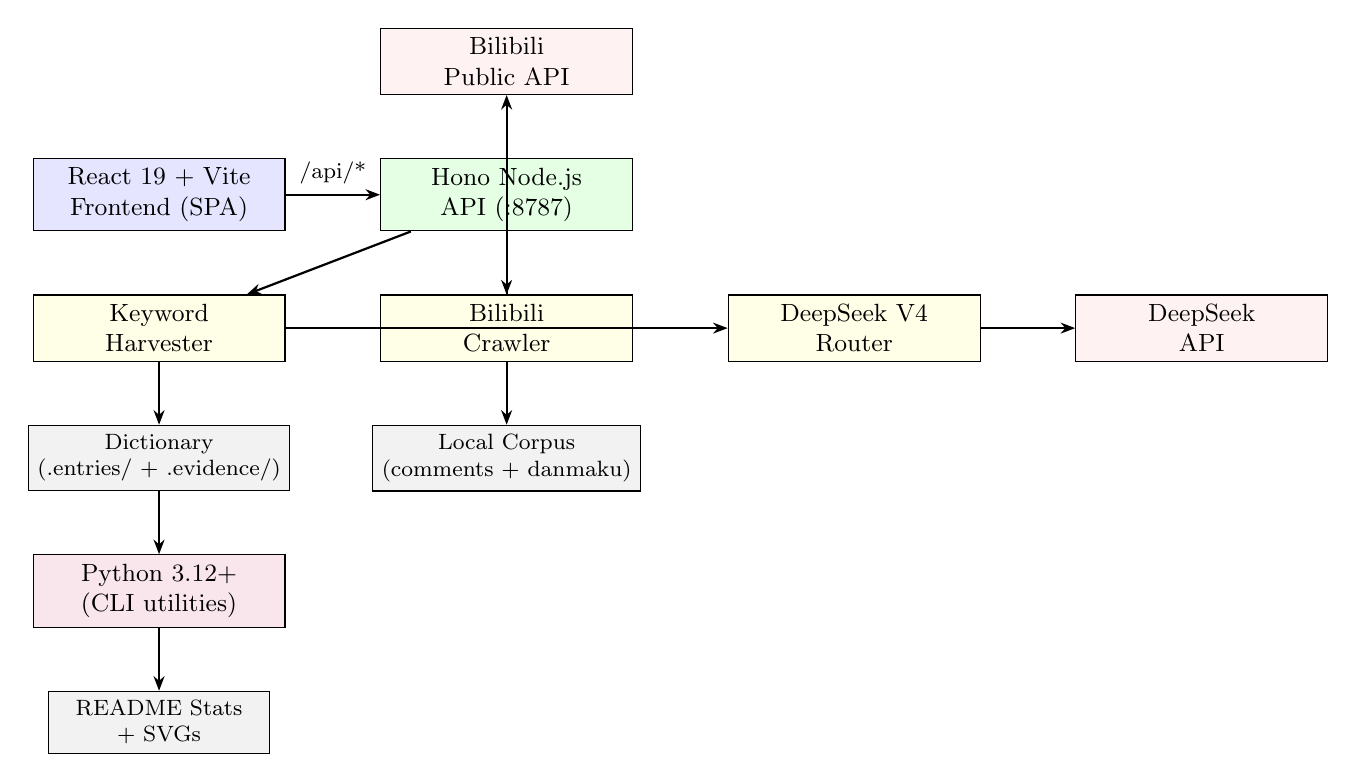
\begin{tikzpicture}[
  node distance=8mm and 12mm,
  box/.style={rectangle,draw,minimum width=32mm,minimum height=8mm,align=center,font=\small},
  databox/.style={rectangle,draw,minimum width=28mm,minimum height=7mm,align=center,font=\footnotesize,fill=gray!10},
  arrow/.style={-{Stealth[scale=0.8]},thick}
]

% Frontend
\node[box,fill=blue!10] (frontend) {React 19 + Vite\\Frontend (SPA)};

% API
\node[box,fill=green!10,right=of frontend] (api) {Hono Node.js\\API (:8787)};

% Services
\node[box,fill=yellow!10,below=of api] (crawler) {Bilibili\\Crawler};
\node[box,fill=yellow!10,left=of crawler] (harvester) {Keyword\\Harvester};
\node[box,fill=yellow!10,right=of crawler] (deepseek) {DeepSeek V4\\Router};

% External
\node[box,fill=red!5,above=of api] (bilibili) {Bilibili\\Public API};
\node[box,fill=red!5,right=of deepseek] (deepseekapi) {DeepSeek\\API};

% Data
\node[databox,below=of harvester] (dict) {Dictionary\\(.entries/ + .evidence/)};
\node[databox,below=of crawler] (corpus) {Local Corpus\\(comments + danmaku)};

% Python
\node[box,fill=purple!10,below=of dict] (python) {Python 3.12+\\(CLI utilities)};

% Output
\node[databox,below=of python] (stats) {README Stats\\+ SVGs};

% Arrows
\draw[arrow] (frontend) -- (api) node[midway,above,font=\footnotesize]{/api/*};
\draw[arrow] (api) -- (crawler);
\draw[arrow] (api) -- (harvester);
\draw[arrow] (crawler) -- (bilibili);
\draw[arrow] (harvester) -- (deepseek);
\draw[arrow] (deepseek) -- (deepseekapi);
\draw[arrow] (harvester) -- (dict);
\draw[arrow] (crawler) -- (corpus);
\draw[arrow] (dict) -- (python);
\draw[arrow] (python) -- (stats);

\end{tikzpicture}
\caption{System architecture diagram. The frontend communicates with the Hono API
  over Vite-proxied HTTP; the API orchestrates Bilibili scraping, dictionary
  harvesting, and DeepSeek validation. Python utilities operate on the
  dictionary and corpus data offline.}
\label{fig:architecture}
\end{figure}

\subsection{Data Flow}

The dictionary pipeline operates as a closed loop:
\begin{enumerate}
  \item Bilibili public API $\rightarrow$ Crawler $\rightarrow$ local comment/danmaku corpus.
  \item Corpus $\rightarrow$ Dictionary Harvester (DeepSeek extracts terms, meanings,
    families; substring + semantic matching locates evidence).
  \item Harvester output $\rightarrow$ split JSON shards (.entries/ + .evidence/).
  \item Coverage Audit reads the dictionary, identifies weak/zero-evidence terms, and
    generates harvest action items.
  \item Action items feed back into the Harvester, closing the loop.
\end{enumerate}

The user analysis path is a separate, read-only flow:
Browser (UID input) $\rightarrow$ Vite proxy $\rightarrow$ Hono API $\rightarrow$
Bilibili API + Dictionary $\rightarrow$ Hybrid Analyzer (DeepSeek + lexicon matching)
$\rightarrow$ JSON response $\rightarrow$ React SPA radar chart + sentence breakdown.

The internal stages of the Hybrid Analyzer---how a user's raw text becomes six-axis
scores---are detailed in Section~6.3.

\subsection{Language Analysis Pipeline}
\label{subsec:pipeline}

Sections~6.1--6.2 describe the system's components and the dictionary-construction loop.
The narrower, user-facing question the system answers is: \emph{given one user's public
utterances, how does raw text become a six-axis behavioral profile?} This subsection traces
that path end to end (Figure~\ref{fig:pipeline}). The pipeline is deliberately split into a
deterministic, fully auditable \emph{lexicon path} and an LLM-based \emph{semantic-judge
path}, merged per the selected analysis mode (Section~3.2). The split is what makes a given
score auditable rather than opaque: every contribution traces back to either a dictionary
entry with quoted evidence or a model judgment with a reasoning trace and quote.

\begin{figure}[htbp]
\centering
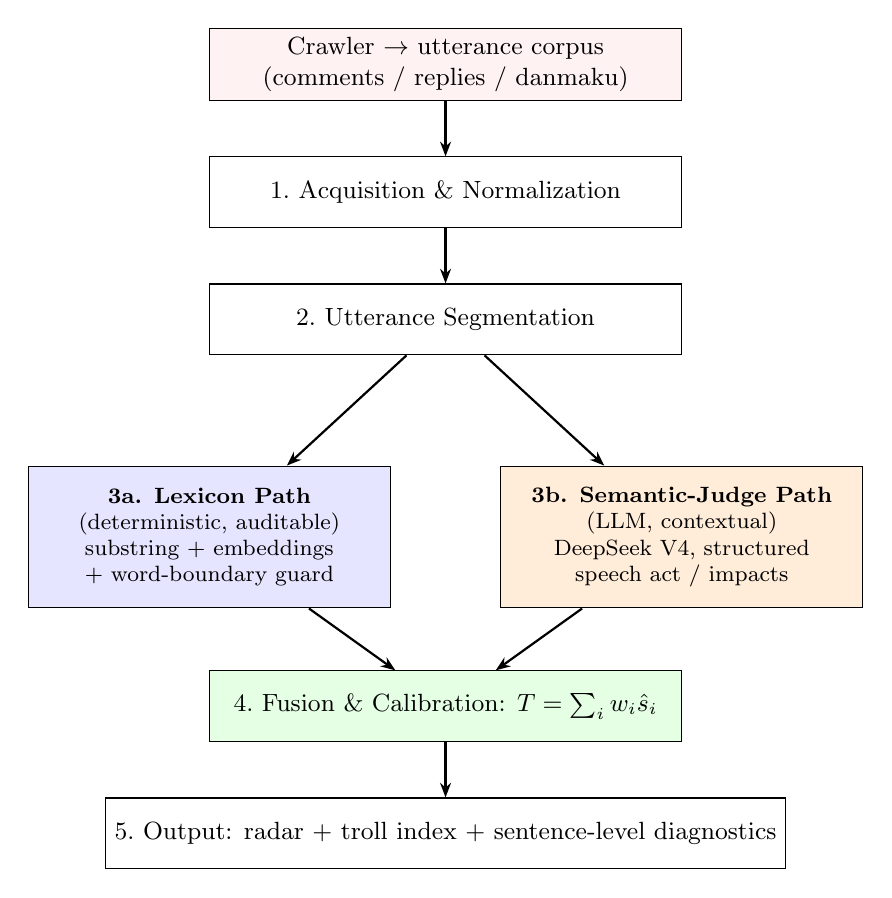
\begin{tikzpicture}[
  node distance=7mm and 10mm,
  box/.style={rectangle,draw,minimum width=60mm,minimum height=9mm,align=center,font=\small},
  pathbox/.style={rectangle,draw,minimum width=46mm,minimum height=18mm,align=center,font=\footnotesize},
  arrow/.style={-{Stealth[scale=0.8]},thick}
]
\node[box,fill=red!5] (crawler) {Crawler $\rightarrow$ utterance corpus\\(comments / replies / danmaku)};
\node[box,below=of crawler] (norm) {1.~Acquisition \& Normalization};
\node[box,below=of norm] (seg) {2.~Utterance Segmentation};
\node[pathbox,fill=blue!10,below=14mm of seg,xshift=-30mm] (lex)
  {\textbf{3a. Lexicon Path}\\(deterministic, auditable)\\substring + embeddings\\+ word-boundary guard};
\node[pathbox,fill=orange!15,below=14mm of seg,xshift=30mm] (judge)
  {\textbf{3b. Semantic-Judge Path}\\(LLM, contextual)\\DeepSeek V4, structured\\speech act / impacts};
\node[box,fill=green!10,below=40mm of seg] (fusion)
  {4.~Fusion \& Calibration: $T = \sum_i w_i \hat{s}_i$};
\node[box,below=of fusion] (out)
  {5.~Output: radar + troll index + sentence-level diagnostics};
\draw[arrow] (crawler) -- (norm);
\draw[arrow] (norm) -- (seg);
\draw[arrow] (seg) -- (lex);
\draw[arrow] (seg) -- (judge);
\draw[arrow] (lex) -- (fusion);
\draw[arrow] (judge) -- (fusion);
\draw[arrow] (fusion) -- (out);
\end{tikzpicture}
\caption{The language-analysis pipeline. The deterministic lexicon path (left) and the LLM
  semantic-judge path (right) run in parallel over each utterance and are fused per the
  selected analysis mode. Every emitted score traces back to a dictionary entry with quoted
  evidence (lexicon) or to a model judgment with a reasoning trace and quote (semantic judge).}
\label{fig:pipeline}
\end{figure}

\textbf{Stage 1 --- Acquisition \& Normalization.} The crawler retrieves the target user's
public comments, replies, and danmaku through the Bilibili API and writes them to the local
corpus under conservative pacing (Section~5.3). Text is re-encoded to a canonical Unicode
form, and the whitespace and newline artifacts that Bilibili injects into multi-line replies
are normalized before analysis.

\textbf{Stage 2 --- Utterance Segmentation.} Because Bilibili frequently bundles several
sentences into a single reply, the analyzer splits each record into \emph{atomic utterances}
--- one logical statement per unit --- so that conflicting signals within one comment are not
averaged into noise. A known trade-off is the loss of cross-paragraph context when a reply is
split aggressively (Section~7.2); segmentation is where single-comment cohesion is exchanged
for per-statement resolution.

\textbf{Stage 3a --- Lexicon Path (deterministic, auditable).} Each utterance is scanned
against all six dictionary families. Matching uses exact substring detection augmented by
three guards: a \emph{word-boundary check} for 1--2 character terms (so the term ``都'' does
not fire inside ``首都''), optional \emph{semantic similarity} against the local embedding
model (\texttt{all-MiniLM-L6-v2}, 384-dimensional vectors) to catch morphological variants
the substring misses, and \emph{meme / quoted-text dampening} so the system does not credit
the user for arguments they merely quote. Every hit contributes evidence to its family's
axis, weighted in proportion to the entry's confidence and accumulated evidence count
(Section~4). Because this path is pure string and vector computation, its output is fully
reproducible and traceable to specific dictionary entries.

\textbf{Stage 3b --- Semantic-Judge Path (LLM).} The full utterance is submitted to DeepSeek
V4 under a \emph{structured-output schema} that forces the model to return, for each relevant
dimension, the \emph{speech act} (e.g., challenge, concession, correction), its \emph{target}
(person vs.\ idea), the speaker's \emph{stance}, a \emph{context role}, and a per-axis
\emph{impact} carrying direction (risk vs.\ positive) and strength ($0$--$1$), together with
a natural-language reasoning trace and a verbatim quote. This path resolves the polysemy,
irony, and meme-dense semantic indirection that defeat substring matching (Section~2.1), at
the cost of being neither deterministic nor free.

\textbf{Stage 4 --- Fusion \& Calibration.} Per-axis scores are produced by fusing the two
paths according to the selected mode: \emph{Hybrid} (lexicon + semantic judge, the default),
\emph{Semantic Judge} (LLM only), or \emph{Lexicon} (dictionary only --- fully auditable, with
no model calls). The four \emph{inverse} axes (evidence sensitivity, logical consistency,
cooperative discussion, correction willingness) are normalized so that \emph{lower = riskier}
before aggregation, and all scores are clamped to $[0, 100]$. The composite trolling index is
the calibrated weighted sum $T = \sum_i w_i \hat{s}_i$, where the dimension weights $w_i$ are
learned by logistic regression over human-labeled examples
(\texttt{python\_backend/analysis/calibration.py}, Section~3.2).

\textbf{Stage 5 --- Output.} The pipeline emits three artifacts: a six-axis radar in which
each axis carries a value, a hand-tuned benchmark, and a human-readable note explaining what
contributed; the composite troll index; and \emph{sentence-level diagnostics} that map each
flagged utterance to its contributing axis impacts and supporting evidence. The diagnostics
are the mechanism that turns a radar-chart point into an inspectable, quotable justification
rather than an opaque number.

\textbf{Why two paths.} Separating the lexicon path from the semantic-judge path is a
deliberate engineering decision rather than an implementation accident. The lexicon path is
cheap, deterministic, and auditable --- every contribution is traceable to a dictionary entry
and a quoted comment --- but it cannot read context. The semantic-judge path reads context
and disambiguates meaning but is non-deterministic and costly. Exposing both and letting the
analysis mode control their blend lets the system trade cost and explainability against
contextual accuracy, and it keeps the auditable path available even when the model is offline
or rate-limited. The two paths are also complementary in failure: a dictionary gap that blinds
the lexicon path is often still caught by the semantic judge, while a model hallucination on
the judge path is bounded by the deterministic lexicon baseline.


% =============================================================================
\section{Current Status and Limitations}

\subsection{Empirical Status}

As of the most recent data snapshot:
\begin{itemize}
  \item \textbf{Corpus size:} 8,972 comments/replies; 153,875 danmaku; 434 timeline data
    points tracking growth over time.
  \item \textbf{Dictionary size:} 4,956 terms across 6 families (attack: 642,
    absolutes: 842, evidence: 861, evasion: 931, cooperation: 868, correction: 812).
  \item \textbf{Coverage ratio:} 0.30\% (15 terms reaching the $\tau = 3$ evidence
    threshold). The dictionary was recently expanded from 1,639 to 4,956 terms; on the
    previous smaller dictionary, coverage was 96\%+. Recovery is in progress through
    the coverage loops.
  \item \textbf{Evidence deficit:} $\Delta = 14,\!806$ additional evidence hits needed
    for full coverage at $\tau = 3$.
\end{itemize}

\subsection{Limitations}

\begin{enumerate}
  \item \textbf{Sample representativeness.} The analysis operates on a bounded public
    comment sample. Users may exhibit different behavior in private messages, on other
    platforms, or in deleted/removed comments that are not accessible via the public API.
  \item \textbf{Language evolution.} Chinese internet slang evolves rapidly. Dictionary
    terms can become obsolete or shift meaning within months. The coverage loops provide
    a mechanism for continuous refresh but require sustained operation.
  \item \textbf{Model dependence.} The semantic judge path depends on DeepSeek V4's
    ability to understand Chinese internet pragmatics. While the model performs well on
    standard Chinese text, it may misclassify highly niche, community-specific in-jokes.
  \item \textbf{Cookie requirement.} The auto-coverage loop requires a valid Bilibili
    session cookie, which imposes a practical barrier for new users and limits
    automated CI/CD integration.
  \item \textbf{Bilingual tooling.} While the documentation and output are bilingual
    (Chinese + English), the underlying analysis pipeline is optimized for Chinese text.
  \item \textbf{Calibration data.} The logistic regression weights $w_i$ in
    Equation~\ref{eq:trolling_index} are learned from human-labeled data. The current
    labeled dataset is small ($n < 100$), limiting confidence in the weight estimates.
\end{enumerate}


% =============================================================================
\section{Future Work}

Several directions would strengthen the system:

\begin{enumerate}
  \item \textbf{Large-scale annotation.} A crowd-sourced or expert annotation campaign
    ($n \geq 1,\!000$) would improve the calibration of the logistic regression weights
    and enable more sophisticated models.
  \item \textbf{Temporal analysis.} Tracking a user's dimension scores over time would
    reveal whether argumentative behavior is stable or context-dependent.
  \item \textbf{Cross-platform generalization.} Adapting the dictionary and scoring
    framework to other Chinese-language platforms (Weibo, Douyin, Zhihu) would test
    the generalizability of the six-dimension model.
  \item \textbf{Semantic matching improvements.} The current local embedding model
    (\texttt{all-MiniLM-L6-v2}) achieves only 27\% recall on Chinese internet slang.
    A domain-adapted or larger multilingual model could improve semantic matching.
  \item \textbf{Automated coverage convergence.} Integrating the three coverage loops
    into a fully autonomous CI/CD pipeline would enable continuous dictionary
    improvement with minimal human intervention.
  \item \textbf{Explainability.} Providing an interactive interface that allows clicking
    on any radar-chart point to see the specific comments and dictionary terms
    that contributed to that score.
\end{enumerate}


% =============================================================================
\section{Conclusion}

We have presented a research prototype for argumentative-behavior risk assessment
on the Bilibili platform. The system combines a theory-grounded six-dimensional
scoring framework with an auditable Chinese internet-slang dictionary and three
iterative coverage loops that progressively close the evidence gap. The hybrid
JS + Python architecture separates real-time user-facing operations from offline
data-heavy work, communicating through JSON contracts. While the current
dictionary coverage is low (0.30\%) following a recent expansion, the coverage-loop
mechanisms provide a principled path to convergence. The system is released as
open-source software under the MIT License at
\url{https://github.com/JunWeiLi233/Bilibili_User_Personality}.


% =============================================================================
% References
% =============================================================================
\begin{thebibliography}{99}

\bibitem{davidson2017automated}
T.~Davidson, D.~Warmsley, M.~Macy, and I.~Weber,
``Automated hate speech detection and the problem of offensive language,''
in \emph{Proc. ICWSM}, 2017.

\bibitem{founta2018unified}
A.~Founta \emph{et al.},
``Large scale crowdsourcing and characterization of Twitter abusive behavior,''
in \emph{Proc. ICWSM}, 2018.

\bibitem{ku2007mining}
L.-W.~Ku, Y.-T.~Liang, and H.-H.~Chen,
``Opinion extraction, summarization and tracking in news and blog corpora,''
in \emph{Proc. AAAI Spring Symposium}, 2007.

\bibitem{dong2006hownet}
Z.~Dong and Q.~Dong,
\emph{HowNet and the Computation of Meaning}.
World Scientific, 2006.

\bibitem{stede2018argumentation}
M.~Stede and J.~Schneider,
``Argumentation mining,''
\emph{Synthesis Lectures on Human Language Technologies},
vol.~11, no.~2, 2018.

\bibitem{peldszus2013argument}
A.~Peldszus and M.~Stede,
``From argument diagrams to argumentation mining in texts,''
\emph{International Journal of Cognitive Informatics and Natural Intelligence},
vol.~7, no.~1, 2013.

\bibitem{kruglanski1996motivated}
A.~W.~Kruglanski and D.~M.~Webster,
``Motivated closing of the mind: `Seizing' and `freezing',''
\emph{Psychological Review}, vol.~103, no.~2, pp.~263--283, 1996.

\bibitem{grice1975logic}
H.~P.~Grice,
``Logic and conversation,''
in \emph{Syntax and Semantics, Vol.~3: Speech Acts},
Academic Press, 1975, pp.~41--58.

\end{thebibliography}

\end{document}
